\documentclass{article}
\NeedsTeXFormat{LaTeX2e}

\ProcessOptions\relax

% fonts
\renewcommand{\rmdefault}{ptm}
\renewcommand{\sfdefault}{phv}


% Language setting
% Replace `english' with e.g. `spanish' to change the document language
\usepackage[russian]{babel}

% Set page size and margins
% Replace `letterpaper' with `a4paper' for UK/EU standard size
\usepackage[letterpaper,top=2cm,bottom=2cm,left=3cm,right=3cm,marginparwidth=1.75cm]{geometry}
\usepackage{wrapfig}
% Useful packages
\usepackage{amsmath}
\usepackage{graphicx}
\usepackage{amssymb}
\usepackage[colorlinks=true, allcolors=blue]{hyperref}
\usepackage{tikz}
\usepackage{titlesec}
\usepackage{mathtools}
\usepackage{cancel}
\usepackage{multicol}
\newcommand{\defeq}{\vcentcolon=}
\usepackage[ruled]{algorithm2e}

\usepackage{arxiv}

\usepackage[utf8]{inputenc} % allow utf-8 input
\usepackage[T1]{fontenc}    % use 8-bit T1 fonts
\usepackage{hyperref}       % hyperlinks
\usepackage{url}            % simple URL typesetting
\usepackage{booktabs}       % professional-quality tables
\usepackage{amsfonts}       % blackboard math symbols
\usepackage{nicefrac}       % compact symbols for 1/2, etc.
\usepackage{microtype}      % microtypography
\usepackage{lipsum}
\usepackage{graphicx}
\graphicspath{ {./images/} }


\title{Разработка эффективных методов построения ансамблевых регрессионных линейных моделей, основанных на максимизации корреляции с откликом}


\author{
 Борисов Иван \\
  Московский государственный университет \\
  имени М. В. Ломоносова  \\
  \texttt{s02210331@gse.cs.msu.ru} \\
}



\begin{document}
\maketitle
\begin{abstract}
В данной статье приведен новый метод построения линейной регрессии, основанный на идее ансамблирования выпуклых комбинаций "элементарных" линейных регрессий, обученных на минимизацию квадратичной ошибки. Каждая выпуклая комбинация (ВПК) строится из принципов максимизации корреляции предсказаний ВПК с целевой переменной, несократимости и нерасширяемости полученной ВПК. Данная линейная модель показывает качество не хуже, чем устоявшееся решение (Эластичная сеть), на данных малого объема, где число объектов имеет тот же порядок, что и число признаков. Результаты работы алгоритма в задаче предсказания параметров химических элементов приведены в таблице [\ref{tbl: 1}].
\end{abstract}

\newpage


\section{Введение}
Пусть дано множество объектов $X = \{x^1, x^2, \dots , x^n\}, x^i \in \mathbb{R}^d$ и множество откликов на них $Y = \{y^1, \dots, y^n\}, y^i \in \mathbb{R}$. Будем решать задачу регрессии, при этом искомое отображение объектов в отклики $a: X \rightarrow Y$ зададим как линейное, то есть  $a(x) = \langle w, x \rangle + b$, где $w \in \mathbb{R}^d, b \in \mathbb{R}$ — обучаемые параметры линейной модели.\\ \\
Для борьбы с мультиколлинеарностью в признаках используются различные виды регуляризации. Если начальная задача задана как $L(\theta) \rightarrow min_{\theta}$, где $\theta = (w, b) \in \mathbb{R}^{d+1}$ — вектор обучаемых параметров, то с добавлением регуляризации новая оптимизационная задача имеет вид \begin{equation}L(\theta) + C(\theta) \rightarrow min_{\theta} \end{equation} где $C: \Theta \rightarrow \mathbb{R}$. \\ \\
Польза регуляризации и способы задания функции $C(\theta)$ рассмотрены в [1-3]. Эксперименты в [3] показали, что регуляризация с использованием Эластичной сети имеет высокую эффективность, но в условиях малого числа объектов результат становится менее стабильным. 
\\ \\
То есть при рассмотрении случая, когда число признаков сопоставимо с числом объектов, треубется более <<сильная>> регуляризация, чем в случае $n>>d$. Исследования в этом направлении представлены в статьях [4-7], основной упор в них делается на модернизации функции регуляризации и отборе признаков на этапе построения модели с помощью итераивных методов построения линеной регрессии. Построенные таким образом модели оказываются более устойчивыми в случае $d >> n$ и обладают лучшим свойством отбора признаков. 
\\ \\
Дальнейшим развитием методово машинного обучения стали методы ансемблирования моделей. В [8] вводятся идея <<стэкинга>> моделей: нахождение оптимальной линейной комбинации $k$ регрессоров с целью улучшения качества предсказания ансамбля относительно предсказания какого-либо $i$-ого предиктора. В [9] вводится алгоритм случайного леса, показавший что ансамблирование моделей с высокой дисперсией и низким смещением приводит к сильному улучшению качества предсказательной способности всего ансамбля.
\\ \\
В [10] идея ансамблирования прикладывается на класс линейных моеделей. Для этого предлагается строить ансамбли из линейных моделей с помощью применения метода случайных подпространст, описанного в [9], и поощрения <<различия>> между полученными линейными моделями. Эксперименты показали, что данный метод дает прирост в метриках по сравнению с обычной линейной регрессией при условии того, что качество каждой отдельно взятой линейной регрессии из ансамбля не превосходит качества обычной регрессии. 
\\ \\
Но в случае высокой размерности признакового пространства качество решения [10] становится менее стабильным. Целью данной работы является обобщение метода, предложенного в [10], в задаче высокой размерности. Достигнуть этого предлагается с помощью идей, схожих с теми, что применялись в [4-7]: усиление регуляризации и итеративный отбор признаков при построении очередной линейной регресии.
\newpage
\section{Постановка задачи}

\subsection{Переход от задачи оптимизации к поиску наилучшей выпуклой комбинации}
Решаем задачу (1). Ее можно переписать в виде оптимизационной задачи с ограничениями:

\begin{equation}
\begin{cases}
    L(\theta) \rightarrow min_\theta \\
    C_1(\theta) \geq 0\\
    \dots \\
    C_k(\theta) \geq 0 \\
\end{cases}
\end{equation}
Если положить $L(\theta) = MSE(\theta) = \sum_{i=1}^n (y^i - b - \langle w, x^i\rangle))^2$ и $C_i = w_i \rho(y, x_i)$, где $\rho(y, x_i)$ — коэффициент корреляции Пирсона, то решение полученной системы:
\begin{equation}
\begin{cases}
    \sum_{i=1}^n (y^i - b - \langle w, x^i\rangle)^2 \rightarrow min_\theta\\
    C_1 = w_1 \rho(y, x_1) \geq 0\\
    \dots \\
    C_k = w_k \rho(y, x_k) \geq 0 \\
\end{cases}
\end{equation}
будет эквивалентно решению построенному по следующему алгоритму (см. [11]):
\begin{enumerate}
    \item Первым делом методом наименьших квадратов строятся $d$ линейных регрессий, которые будем называть <<элементарными>> регрессорами:
    $$
    R_i = b_i + w_ix_i 
    $$
    $$
    \overline{R} = (R_1, \dots, R_d)
    $$
    \item Далее находится выпуклая комбинация, имеющая максимальную корреляцию с откликом:
    $$
    \forall \overline{c} = (c_1, \dots, c_d) : \sum_{i=1}^d c_i = 1, c_i \geq 0 \Rightarrow \rho(P(\overline{c}^*, \overline{R}), y) \geq \rho(P(\overline{c}, \overline{R}), y),
    $$
    $$
    \text{где } \overline{c}^* \text{- вектор оптимальной выпуклой комбинации}, P(\overline{c},\overline{R}) = \sum_{i=1}^d c_iR^i
    $$
    \item Далее с помощью метода наименьших квадратов строится линейная регрессия для прогнозирования $y$ по выпуклой комбинации $P(\overline{c}^*, \overline{R})$:
    $$
    a(x) = \beta + \alpha P(\overline{c}^*, \overline{R})
    $$
\end{enumerate}
Итого, с помощью $C_i = w_i \rho(y, x_i)$ потребовали, чтобы знаки $i$-ого веса модели и коэффициента корреляции $i$-ой переменной с целевой переменной совпадали - задали регуляризацию. С помощью линейного преобразования, описанного в последнем шаге алгоритма, повышаем дисперсию между <<элементарными>> регрессорами, что положительно сказывается на общей предсказательной способности ансамбля (см. [11]). Далее задачу поиска оптимальной выпуклой комбинации во втором шаге предлагается решать итерративно с помощью <<несократимых>> и <<нерасширяемых>> комбинаций, определения которых будут введены позднее,  благодаря этому задается дополнительное свойство <<селективности>> (отбора признаков) для построенной модели.
\newpage

\subsection{Коэффициент Пирсона для выпуклой комбинации <<элементарных>> регрессоров}
Ключевую роль в построении алгоритма играет коэффициент Пирсона:

\begin{equation}
    \rho(X, Y) = \frac{cov(X, Y)}{\sqrt{\mathbb{D}X} \sqrt{\mathbb{D}Y}}, \text{ где } cov(X, Y) = \mathbb{E}[(X - \mathbb{E}X)(Y - \mathbb{E}Y)]
    \label{formula:3}
\end{equation} \\
Для произвольной регрессии $R$, построенной методом наименьших квадратов, известно:

\begin{equation}
    \mathbb{E}R = Y \text{ и } cov(Y, R) = \mathbb{D}R
    \label{formula:4}
\end{equation} 
Также в [11] было выведено разложение для дисперсии выпуклой комбинации случайных функций \overline{Z} = $(Z_1, \dots, Z_l)$ с коэффициентами $\overline{c} = (c_1, \dots, c_l), \sum_i c_i = 1:$
\begin{equation}   
    \mathbb{D}P(\overline{Z}) = \sum_{i=1}^l c_i \mathbb{D}Z_i - \frac{1}{2} \sum_{i=1}^l \sum_{j=1}^l c_i c_j \varrho(Z_i, Z_j),
    \label{formula:5}
\end{equation}
$$
\text{где } \varrho(Z_i, Z_j) = \mathbb{E}(Z_i - \mathbb{E}Z_i - Z_j + \mathbb{E}Z_j)^2 
$$
Таким образом, объединив (\ref{formula:3}), (\ref{formula:4}), (\ref{formula:5}) имеем:
\begin{equation}
    \rho(Y, P(\overline{c}, \overline{R})) = \frac{\sum_{i=1}^d c_iR_i}{\sqrt{\mathbb{D}Y} \sqrt{ \sum_{i=1}^l c_i \mathbb{D}R_i - \frac{1}{2} \sum_{i=1}^l \sum_{j=1}^l c_i c_j \varrho(R_i, R_j)}}, 
    \label{formula:6}
\end{equation}

$$
\text{где } \varrho(R_i, R_j) = \mathbb{E}(R_i - R_j)^2 
$$
\subsection{Основные понятия}
Определим следующие множества: \\
$$
\overline{D}_d = \{\overline{c}: \sum_{i=1}^d c_i = 1, c_i \geq 0\}, D_d = \{\overline{c} :\sum_{i=1}^d c_i = 1, c_i > 0\}
$$
\textbf{Определение 1}: Ансамбль предикторов $\overline{r} = \{r_1, \dots, r_d\}$ называется \textit{несократимым относительно коэффициента корреляции}, если выполнено одно из двух требований: \\
$$\text{1. } d = 1 \text{ и } \rho(Y, r_1) > 0$$
$$\text{2. } d > 1 \text{ и } \exists c^* \in D_d: \forall c \in \overline{D}_d \textbackslash D_d \Rightarrow \rho(Y, P(\overline{r}, c^*)) \geq \rho(Y, P(\overline{r}, c))$$
\textbf{Определение 2}: Несократимый ансамбль $\overline{r} = (r_1, \dots, r_d)$ будем называть \textit{нерасширяемым несократимым ансамблем (ННА)}, если $\not\exists $ несократимого ансамбля $\overline{r}^* = (r_1, \dots, r_{d+1}): \forall r_i \in \overline{r} \Rightarrow r_i \in \overline{r}^*$. \\ \\
\textbf{Утверждение:} 
В [11] было доказано существование ННА $r^* \subseteq \overline{R}: \rho(r^*, c^*) = \underset{\underset{\overline{r} \subseteq \overline{R}}{c \in \overline{D}_d}}{\max} \rho (Y, P(\overline{r}, c))$.
\newpage
\subsection{Необходимые условия оптимальности выпуклой комбинации}
Введем обозначение: $W(\theta) = \{c \in \mathbb{R}^d | \sum_{i=1}^d c_i \mathbb{D}[r_i] = \theta, \sum_{i=1}^{d} c_i = 1, c_i \geq 0\}$ \\ \\
Рассмотрим двумерный случай $d=2$ и пусть $\mathbb{D}r_1 > \mathbb{D}r_2$: \\
\begin{equation}
\centering
\begin{cases}
    c_1 \mathbb{D}(r_1) + c_2 \mathbb{D}(r_2) = \theta \\
    c_1 + c_2 = 1
\end{cases}
\Rightarrow
\begin{cases}
    c_1 = \frac{\theta - \mathbb{D}r_1}{\mathbb{D}r_1 - \mathbb{D}r_2} \\
    \\
    c_2 = \frac{\mathbb{D}r_2 - \theta}{\mathbb{D}r_1 - \mathbb{D}r_2}
\end{cases}
\label{formula:7}
\end{equation}
Тогда $c \in D_2 \Leftrightarrow \theta \in (\mathbb{D}r_2, \mathbb{D}r_1)$. \\ \\
Теперь вспомним, что мы хотим максимизировать корреляцию с откликом, поэтому, пользуясь формулой (\ref{formula:6}):
$$
\rho(Y, P(r, \theta)) = \frac{\theta}{\sqrt{\mathbb{D}Y} \sqrt{ \theta + \varrho(r_1, r_2) \frac{(\theta - \mathbb{D}r_1)(\theta - \mathbb{D}r_2)}{(\mathbb{D}r_1 - \mathbb{D}r_2)^2} }} \rightarrow max_\theta
$$ \\
Взяв производную по $\theta$ и приравняв ее к $0$, получим: \\
\begin{equation}
    \theta^* = \frac{-2 \varrho(r_1, r_2) \mathbb{D}r_1 \mathbb{D} r_2}{(\mathbb{D}r_1 - \mathbb{D}r_2)^2 - \varrho(r_1, r_2)(\mathbb{D}r_1 + \mathbb{D} r_2)}
    \label{formula:8}
\end{equation}
\\
\textbf{Утверждение 1:} \\ Ансамбль $\overline{r} = (r_1, r_2)$ является несократимым $\Rightarrow$ 
\begin{cases}
    \theta^* = \frac{-2 \varrho(r_1, r_2) \mathbb{D}r_1 \mathbb{D} r_2}{(\mathbb{D}r_1 - \mathbb{D}r_2)^2 - \varrho(r_1, r_2)(\mathbb{D}r_1 + \mathbb{D} r_2)} \\
    \\
    \theta^* \in (\mathbb{D}r_1, \mathbb{D}r_2) \\ \\
    \exists i \in \{1, 2\}: \rho(Y, P(r, \theta^*)) \geq \rho(Y, r_i) 
\end{cases}\\ \\ \\
При переходе от двумерного случая к $d$-мерному необходимое условие несократимости ансамбля $\overline{r} = (r_1, \dots, r_d)$ относительно коэффициента корреляции принимает вид утверждения 2.\\ \\
\textbf{Утверждение 2:}
$r = (r_1, \dots, r_d)$ - несократимый $\Rightarrow \exists \theta > 0: Q(\theta) = \sum_{i=1}^d \sum_{j=1}^d c_i c_j \varrho(r_i, r_j)$ достигает строгого максимума на $W(\theta)$ в точке $c^* = (c_1^*, \dots, c_d^*), c_i^* > 0$. \\ \\
Доказательство приведено в [11]. \\ \\
Тогда \\
\begin{equation}
\begin{cases}
    Q(\theta) \rightarrow max_{\theta}\\
    \sum_{i=1}^d c_i = 1\\
    \sum_{i=1}^{d} c_i \mathbb{D}r_i = \theta
\end{cases}
\Leftrightarrow 
\centering
\begin{cases}
    \frac{\partial L}{\partial c_k}\big\vert_{c^*} = 0 \\ \\
    \frac{\partial {L}}{\partial \mu}\big\vert_{c^*} = 0 \\ \\
    \frac{\partial {L}}{\partial \lambda}\big\vert_{c^*} = 0, 
\end{cases}
\centering
\label{formula:9}
\end{equation}
здесь 
$L (c, \lambda, \mu) = \sum_{i=1}^d \sum_{j=1}^d c_i c_j \varrho(r_i, r_j) + \lambda \bigg(\sum_{i=1}^{d} c_i \mathbb{D}r_i - \theta \bigg) + \mu \bigg(\sum_{i=1}^d c_i - 1\bigg) 
$ — лагранжиан.
\\
Переписав (\ref{formula:9}) в матричном виде получаем: \\
$$
\begin{cases}
    \overline{c}^*P + \lambda V + \mu I = O \\
    \overline{c}^* V = \theta\\
    \overline{c}^*I = 1,
\end{cases} 
$$
где 
$
P = \big\vert \big\vert \rho(r_i, r_j) \big\vert \big\vert_{d \times d}, V = \big\vert \big\vert \mathbb{D} r_i \big\vert \big\vert_{1 \times d}, I = \big\vert \big\vert 1 \big\vert \big\vert_{1 \times d}, O = \big\vert \big\vert 0 \big\vert \big\vert_{1 \times d}
$ \\ \\
Рассмотрим случай $\exists P^{-1}$:
$$
\begin{cases}
    (\overline{c}^*)^T + \lambda P^{-1} V + \mu P^{-1} = O \\
    \overline{c}^* V = \theta\\
    \overline{c}^*I = 1,
\end{cases} 
\Rightarrow
\begin{cases}
    \theta + \lambda \underbrace{V^T P^{-1} V}_{\alpha} + \mu \underbrace{V^T P^{-1}I }_{\beta} = O \\
    1 + \lambda \underbrace{I^T P^{-1}V}_{\beta} + \mu \underbrace{I^T P^{-1}I}_{\gamma} = O
\end{cases} 
\Rightarrow
\begin{cases}
    \theta + \lambda \alpha + \mu \beta = O \\
    1 + \lambda \beta + \mu \gamma = O
\end{cases} 
$$
Отсюда:
$$
\begin{cases}
    \lambda = \frac{\beta - \theta \gamma}{\alpha \gamma - \beta^2} \\ \\
    \mu = \frac{\alpha - \theta \beta}{\beta^2- \alpha \gamma}
\end{cases}
$$
Итого:
$$
(c^*)^T  + \frac{\beta - \theta \gamma}{\alpha \gamma - \beta^2} P^{-1}V + \frac{\alpha - \theta \beta}{\beta^2- \alpha \gamma} P^{-1} = O
$$
В скалярном виде: \\
$$
c_k^* = \frac{\theta \gamma - \beta}{\alpha \gamma - \beta^2} \sum_{i=1}^d P^{-1}_{ki}\mathbb{D}r_i + \frac{\theta \beta - \alpha}{\beta^2- \alpha \gamma} \sum_{i=1}^d P^{-1}_{ki}
$$
Обозначим: \\
$$
A_k = \sum_{i=1}^l P^{-1}_{ki}\mathbb{D}r_i, B_k = \sum_{i=1}^l P^{-1}_{ki}
$$
$$
C_k = \frac{\alpha B_k - \beta A_k}{\alpha \gamma - \beta^2}, D_k = \frac{\gamma A_k - \beta B_k}{\alpha \gamma - \beta^2}
$$
Тогда: \\
\begin{equation}
    \boxed{c_k^* = C_k + D_k \theta}
    \label{formula:10}
\end{equation}

Теперь, чтобы получить необходимые условия несократимости ансамбля, необходимо ввести еще несколько обозначений: \\
$$
Q_0 = \sum_{i=1}^{d} \sum_{j=1}^{d} C_i C_j \varrho_{ij}, Q_1 = \sum_{i=1}^{d} \sum_{j=1}^{d} (C_i D_j  + C_j D_i)\varrho_{ij}, Q_2 = \sum_{i=1}^{d} \sum_{j=1}^{d} D_i D_j \varrho_{ij}
$$
$$
\kappa(\theta) = \frac{\theta}{\sqrt{(1- 0.5 Q_1)\theta - 0.5 Q_2 \theta^2 - 0.5 Q_0}}
$$
Пользуясь (\ref{formula:6}), имеем:
$$
\rho(Y, P(\overline{r}, c^*)) = \frac{\kappa(\theta)}{\mathbb{D}Y}
$$
И теперь необходимое условие несократимости ансамбля $\overline{r} = (r_1, \dots, r_d)$ относительно отклика можно задать в виде утверждения 3. \\ \\
\textbf{Утверждение 3:} Если ансамбль $\overline{r}$ является несократимым относительно коэффициента корреляции, и \exists $P^{-1}$, $(\theta_{min}, \theta_{max})$ — интервал значений, на котором $\forall k = 1, \dots, d \Rightarrow c^*_k > 0$, тогда выполнены неравенства: \\
$$
\begin{cases}
    \theta_{min} < \theta^* < \theta_{max} \\
    \kappa(\theta^*) > \kappa(\theta_{min}) \\ 
    \kappa(\theta^*) > \kappa(\theta_{max}), 
\end{cases}
$$
$$\text{где } c_k^* = C_k + D_k \theta, \theta^* = \frac{Q_0}{(1- 0.5 Q_1)}$$
Также максимум корреляции $\rho(Y, P(\overline{r}, c)) = \frac{\kappa(\theta)}{\mathbb{D}Y}$ на $\overline{D}_d$ достигается при $\theta^*$ в точке $c^*$. \\ \\
Доказательство данного утверждения было приведено в [11].
\subsection{Итог}
Утверждения 2 и 3 позволяют итеративно наращивать число предикторов таким образом, что полученная в итоге комбинация будет обладать свойством нерасширяемости и несократимости. Это гарантирует достижение максимума корреляции построенной комбинации с целевой переменной.
\section{Программная реализация}
\subsection{Полный алгоритм}
Приведем краткий алгоритм работы программы.
\subsubsection{Случай 2 <<элементарных>> регрессоров}
\begin{itemize}
    \item Обучаем $d$ регрессий, каждую на своем i-ом признаке с помощью метода наименьших квадратов.
    \item На валидационной выборке оцениваем дисперсии и расстояния по формулам: $$
    \mathbb{D}R_i = \frac{1}{n} \sum_{k=1}^n (R_i(x^k_i) - \mathbb{E}R_i)^2, \mathbb{E}R_i = \frac{1}{n} \sum_{k=1}^n R_i(x^k_i), \varrho(R_{i}, R_{j}) = \frac{1}{n} \sum_{k=1}^n (R_i(x^k_i) - R_j(x^k_j))
    $$
    \item Вычисляем $\theta^*$ для всех пар <<элементарных>> предикторов по формуле (\ref{formula:9}).
    \item В соответствии с утверждением 1:
    \subitem - Проверяем $\theta^*_{i,j} \in (\mathbb{D}R_i, \mathbb{D}R_j)$.
    \subitem - Оцениваем корреляции с откликом отдельных предикторов как: 
    $$
        \rho(Y, r_i) = \sqrt{\frac{\mathbb{D}R_i}{\mathbb{D}Y}}
    $$
    \subitem - По формуле (\ref{formula:6}) оцениваем корреляцию из пар <<элементарных>> предикторов.
    \subitem - Оставляем только те $\theta^*_{ij}$, для которых $\forall k \in \{i, j\}: \rho(Y, P(\overline{R}, \theta_{ij}^*)) \geq \rho(Y, R_k)$ (корреляция Пирсона полученной комбинации выше, чем у предикторов по отдельности).
\end{itemize}
По итогу имеем матрицу: \\
$$
\Theta^* = 
\begin{cases}
    \theta^*_{ij}, \text{вып. утверждение 1} \\
    0, \text{иначе}
\end{cases}
$$
\subsubsection{Основной алгоритм}
\label{algorithm}
\begin{itemize}
    \item Создаем словарь, ключами которого являются индексы <<элементарных>> регрессоров уже включенных в несократимый ансамбль, значениями — соответсвующие им веса $c^*_k$.
    \item Для каждого ненулевого $\theta^*_{ij}$ \in $\Theta^*, i \leq j$ по формуле (\ref{formula:7}) находим коэффициенты выпуклой комбинации и записываем полученную пару в словарь. Далее для каждой комбинации запускаем цикл описанный ниже.
    \subitem - Идем в цикле по переменным, не вошедшим в текущий несократимый ансамбль, и добавляем соответсвующей переменной элементарный предиктор в ансамбль.
    \subitem - Проверяем выполнимость условий утверждения 3 для полученного ансамбля:
    \subitem - Если условия выполнены, удаляем из словаря предыдущий несократимый ансамбль и добавляем новый, расширенный. И запускаем перебор новых переменных для него.
    \subitem - Если хотя бы одно из условий утверждения 3 нарушено, то завершаем перебор для данного ансамбля, возвращаемся к циклу перебора индексов для предыдущего несократимого ансамбля.    
\end{itemize} \\
В результате данного алгоритма имеем словарь вида: индексы предикторов $\leftrightarrow$ веса выпуклой комбинации. Чтобы получить окончательный результат, для каждой комбинации вычисляем предсказание и каким-либо образом <<усредняем>> по всем комбинациям.
\subsection{Альтернативный алгоритм}
Вместо перебора всевозможных комбинаций на каждом шаге будем отбирать максимально скоррелированную с целевеой переменной комбинацию. Для этого предлагается строить элементарные предикторы аналогично тому, как это делается в методе случайного леса, то есть с использованием бутстрэпа и метода случайных подпространств. Все остальные условия несократимости и нерасширяемости остаются неизменными.
\section{Эксперименты}
Сравним полученную модель с существующими решениями на реальных данных.
\subsection{Данные}
Даны 2 датасета размерами $176 \times 94$ и $92 \times 100$, содержащие различные химические элементы. К примеру, CaAuBi, CdAgSb, CdAuSb, CdCuSb, CePdBi, ..., ZrNiSn, ZrPdSn, ZrPtSn, ZrRhSb, ZrRuSb. Предлагается по набору признаков химических элементов предсказать некоторый параметр данного химического элемента, в данных они названы <<a, A>>, <<c, A>>.

\subsection{Используемые модели}
Для сравнения будут использоваться линейные регрессии $a(x) = \langle w, x \rangle + b$, минимизирующие MSE, с различными функциями регуляризации. Если $L = \sum_{i=1}^n (y_i - a(x_i))^2 + R(w)$, то в зависимости от функции $R(w)$ определим:
\begin{itemize}
    \item Ridge: $R(w) = ||w||_2^2$
    \item Lasso: $R(w) = ||w||_1$
    \item ElasticNet: $R(w) = 0.5 \cdot ||w||_1 + 0.25 \cdot ||w||_2^2$
\end{itemize}
Также для сравнения обучим ARD-регрессию [14] и Байесовскую Ridge регрессию [15]. \\ \\
Сравнивать будем модель, построенную на выпуклых комбинациях (ВПК). Для добавления нового предиктора использовалось условие, при котором коэффициент корреляции новой комбинации превосходит коэффициент корреляции предыдущей ВПК в $\tau_{irr} = 1.25$ раз.
\\
Рассмотрим различные методы усреднения полученного ансамбля. За $l$ обозначим число выпуклых комбинаций; $\text{ВПК}_i(x)$ - предсказание i-ой комбинации на x; y - целевая переменная, соответствующая x; Y - целевые переменные тренировочной выборки; $\overline{\text{ВПК}}(X)$ - матрица, столбцы которой - предсказания каждой выпуклой комбинации на тренировочном датасете; $\rho_i$ - коэффициент корреляции Пирсона i-ой комбинации с целевой переменной на обучающей выборке, тогда введем:
\begin{itemize}
    \item $\text{ВПК}_{\text{ср}}(x) = \alpha_1 (\frac{1}{l} \sum_{i=1}^l \text{ВПК}_i(x)) + \beta_1$
    \item $\text{ВПК}_{\text{кор}}(x) = \alpha_2 ( \sum_{i=1}^l \frac{1}{1 - \rho^2_i} \text{ВПК}_i(x)) + \beta_2$
    \item $\text{ВПК}_{\text{лин}}(x) = \langle \arg \min_{\theta \in \mathbb{R}^l} MSE(\overline{\text{ВПК}}(X) \cdot \theta, Y), x \rangle$
\end{itemize}
где $\alpha_i, \beta_i$ — коэффициенты, подобранные по MSE на тренировочной выборке.
\\ \\
Также рассмотрим метод построения оптимальных выпуклых комбинаций на бутстрапированных выборках с использованием метода случайных подпространств при построении очередного предиктора. Введем 2 дополнительных параметра $n_{\text{bootstrap}}$ — число бутстрапирований, $p$ - вероятность вхождения $i$-ого признака в методе случайных подпространств. Обучим модели, зафиксировав $seed$ и параметры $n_{\text{bootstrap}} = 10$ и $p=0.5$.
\newpage
\subsection{Результаты}
Разобьем данные на обучение/тест в соотношении 8:2, зафиксировав  $random\_state=42$. Получим соотношения 140/36, 73/19 на обучение и тестирование для первого и второго набора данных соответственно. Через ВПК$_{\text{ср}}$, ВПК$_{\text{кор}}$, ВПК$_{\text{лин}}$ обозначим различные способы усреднения финальных моделей, через $/$ отделим метрику модели полного перебора и модели, построенной на бутстрапировании обучающей выборки.
\begin{center}
\begin{table}[!htb]
\begin{tabular}{c c}
     \begin{tabular}{||c | c | c||}
 \hline
 Модель & $r^2$ & Корреляция
  \\
   & & 
 Пирсона \\[0.5ex] 
 \hline\hline
 \text{ВПК}_{\text{ср}} & 0.5655/0.89 & 0.7938/0.9461 \\ 
 \hline
 \text{ВПК}_{\text{кор}} & 0.5977/0.894 & 0.8099/0.9485 \\ 
 \hline
 \text{ВПК}_{\text{лин}} & 0.9527/0.9176 & 0.9766/0.9623 \\ 
 \hline
 Ridge & \textbf{0.9603} & \textbf{0.9809} \\
 \hline
 Lasso & 0.8427 & 0.9224\\
 \hline
 ElasticNet & 0.8849 & 0.9427  \\
 \hline
 ARD & 0.9111 & 0.9581\\ [1ex] 
 \hline
 Байесовская & 0.9438 & 0.9727 \\
  \hline
\end{tabular} &  

\begin{tabular}{||c | c | c||}
 \hline
 Модель & $r^2$ & Корреляция
  \\
   & & 
 Пирсона \\[0.5ex] 
 \hline\hline
 \text{ВПК}_{\text{ср}} & 0.8993/0.9238 & 0.9489/0.9624 \\ 
 \hline
 \text{ВПК}_{\text{кор}} & 0.8815/0.9207 & 0.9389/0.9605 \\ 
 \hline
 \text{ВПК}_{\text{лин}} & 0.9613/0.9348 & 0.9814/0.97 \\ 
 \hline
 Ridge & 0.9611 & 0.9810 \\
 \hline
 Lasso & 0.9492 & 0.9750 \\
 \hline
 ElasticNet & 0.9527 & 0.9766  \\
 \hline
 ARD & \textbf{0.9627} & \textbf{0.9822}\\ [1ex] 
 \hline
 Байесовская & 0.9624 & 0.9821 \\
  \hline
\end{tabular}
\end{tabular}
\\
\label{tbl: 1}
\caption{Сравнение качества линейных регрессий}
\end{table}
\end{center}
По результатам таблицы [\ref{tbl: 1}] можно судить о том, что лучшее качество показывает третий метод усреднения классического алгоритма, при этом первый и второй методы усреднений слишком сильно теряют в качестве. Далее сравнение ВПК с другими моделями будет проводиться по лучшему из результатов. Полученный алгоритм имеет качество выше, чем Лассо и Эластичная сеть, которая является устоявшимся решением в задаче высокой размерности. При этом высокий результат показывает Ridge, с ARD и Баейсовской регрессиями паритет. В целом новый метод имеет право на существование и может показывать результаты не хуже устоявшихся решений. 
\subsection{Анализ моделей}
Рассмотрим классическую ВПК модель. Для этого построим распределение длин комбинаций и коэффициента Пирсона на обучающей выборке.
\begin{figure}[!htb]
    \centering
    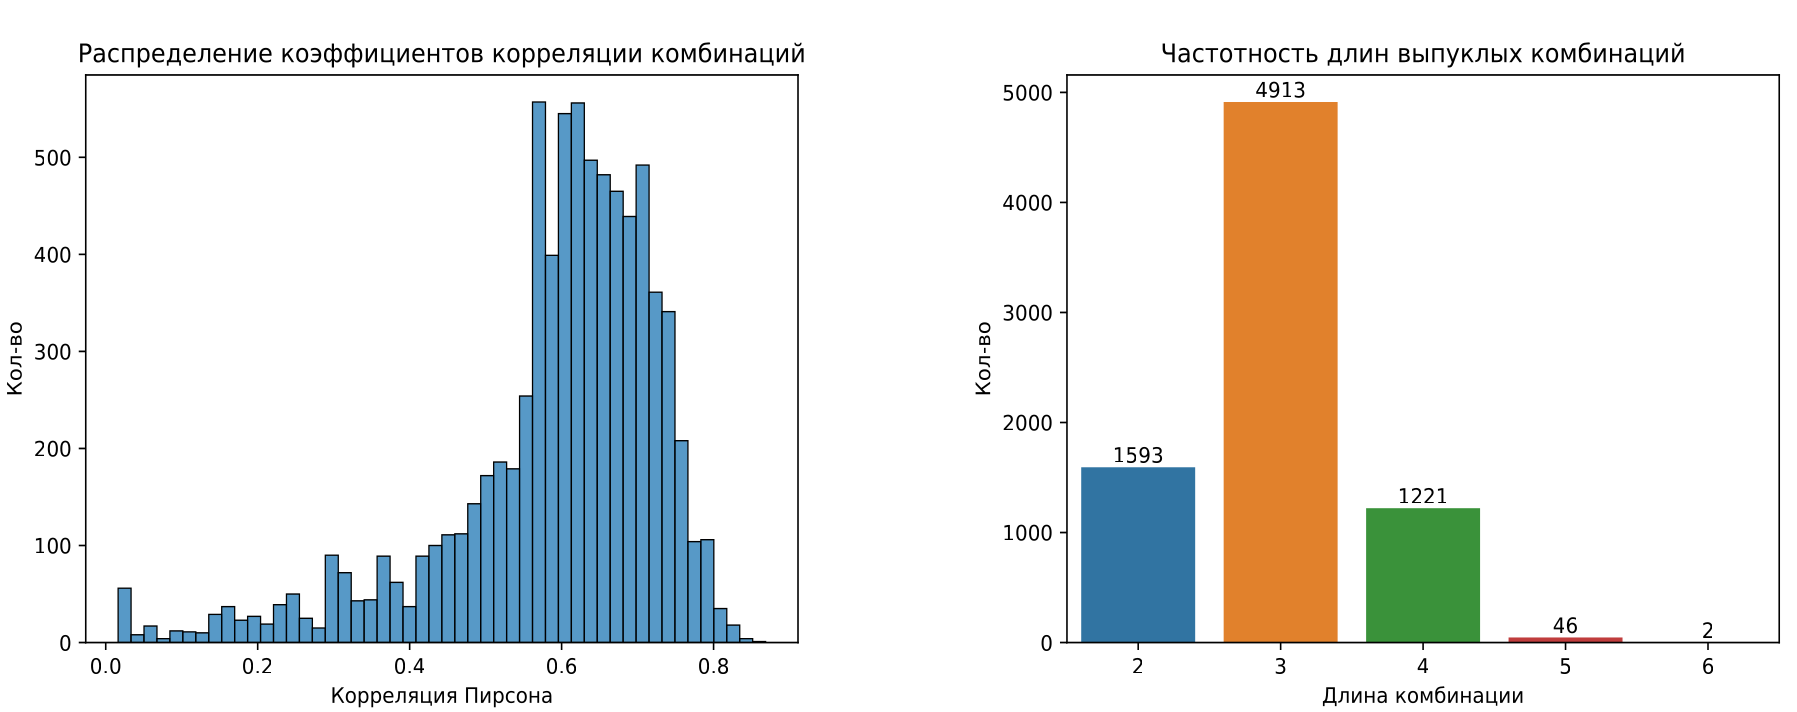
\includegraphics[width=1\linewidth]{pictures/pic1.png}
    \caption{ВПК на первом наборе данных}
    \label{pic 1}
\end{figure}
\newpage
\begin{figure}[!htb]
    \centering
    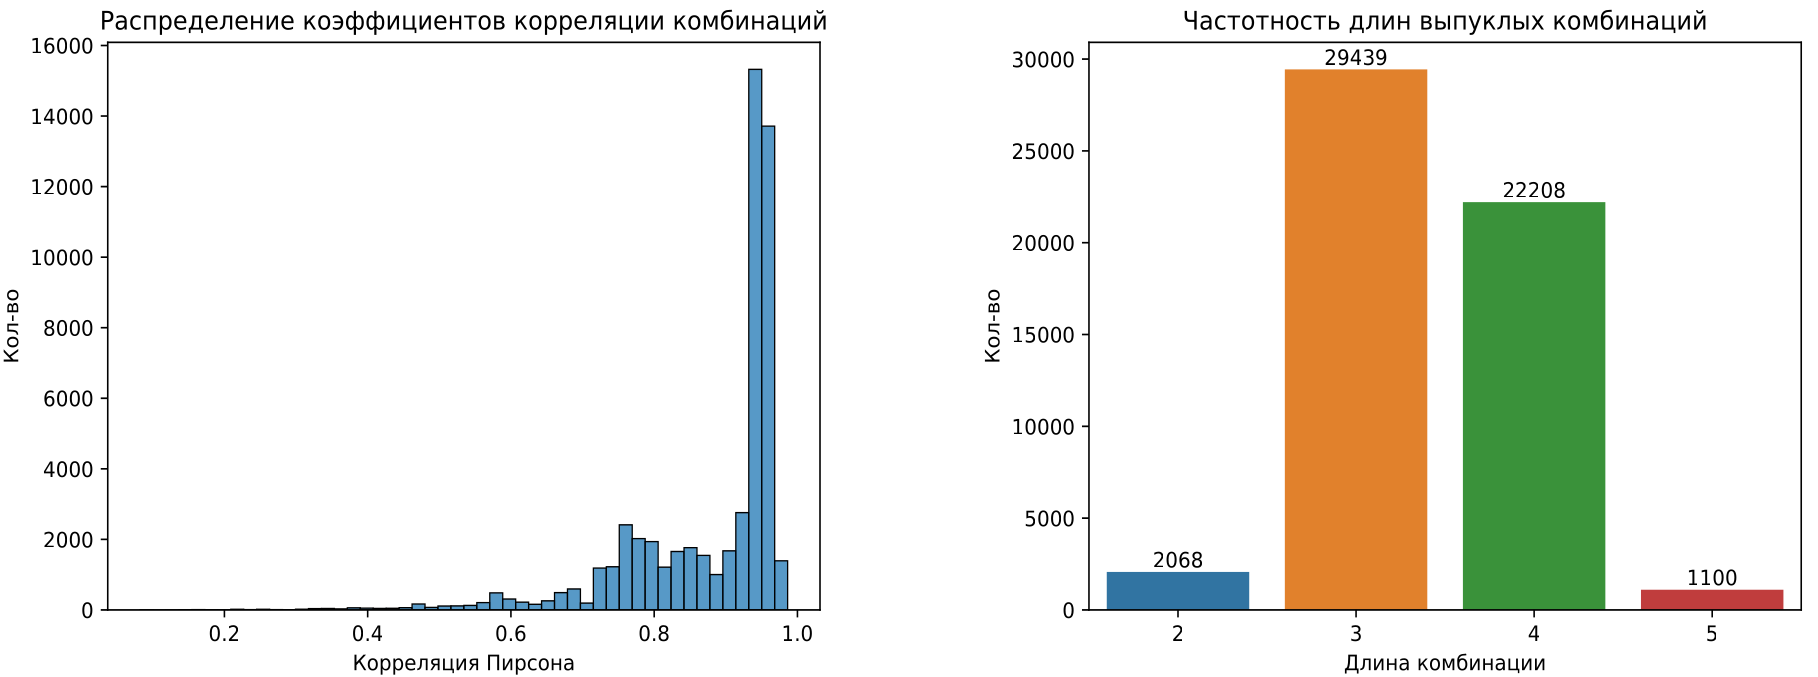
\includegraphics[width=1\linewidth]{pictures/pic2.png}
    \caption{ВПК на втором наборе данных}
    \label{pic 2}
\end{figure}
Из графиков [\ref{pic 1}] и [\ref{pic 2}] можно видеть, что коэффициент корреляции ВПК выше, чем у каждого из предикторов. При этом алгоритм не склонен находить длинные комбинации, однако данное свойство можно регулировать варьируя параметр $\tau_{irr}$ - параметр роста коэффициента корреляции Пирсона. \\ \\
Рассмотрим, с какой скоростью растет количество уникальных предикторов в альтернативном методе построения ВПК с применением метода случайных подпространств. По оси $x$ отложим число бустрапированных выборок, по оси $y$ — число уникальных предикторов. Параметр $p$ — вероятности вхождения признака в построение очередного предиктора — зафиксируем равным 0.5. Далее все графики будут приведены для обоих наборов данных.
\begin{figure}[!htb]
    \centering
    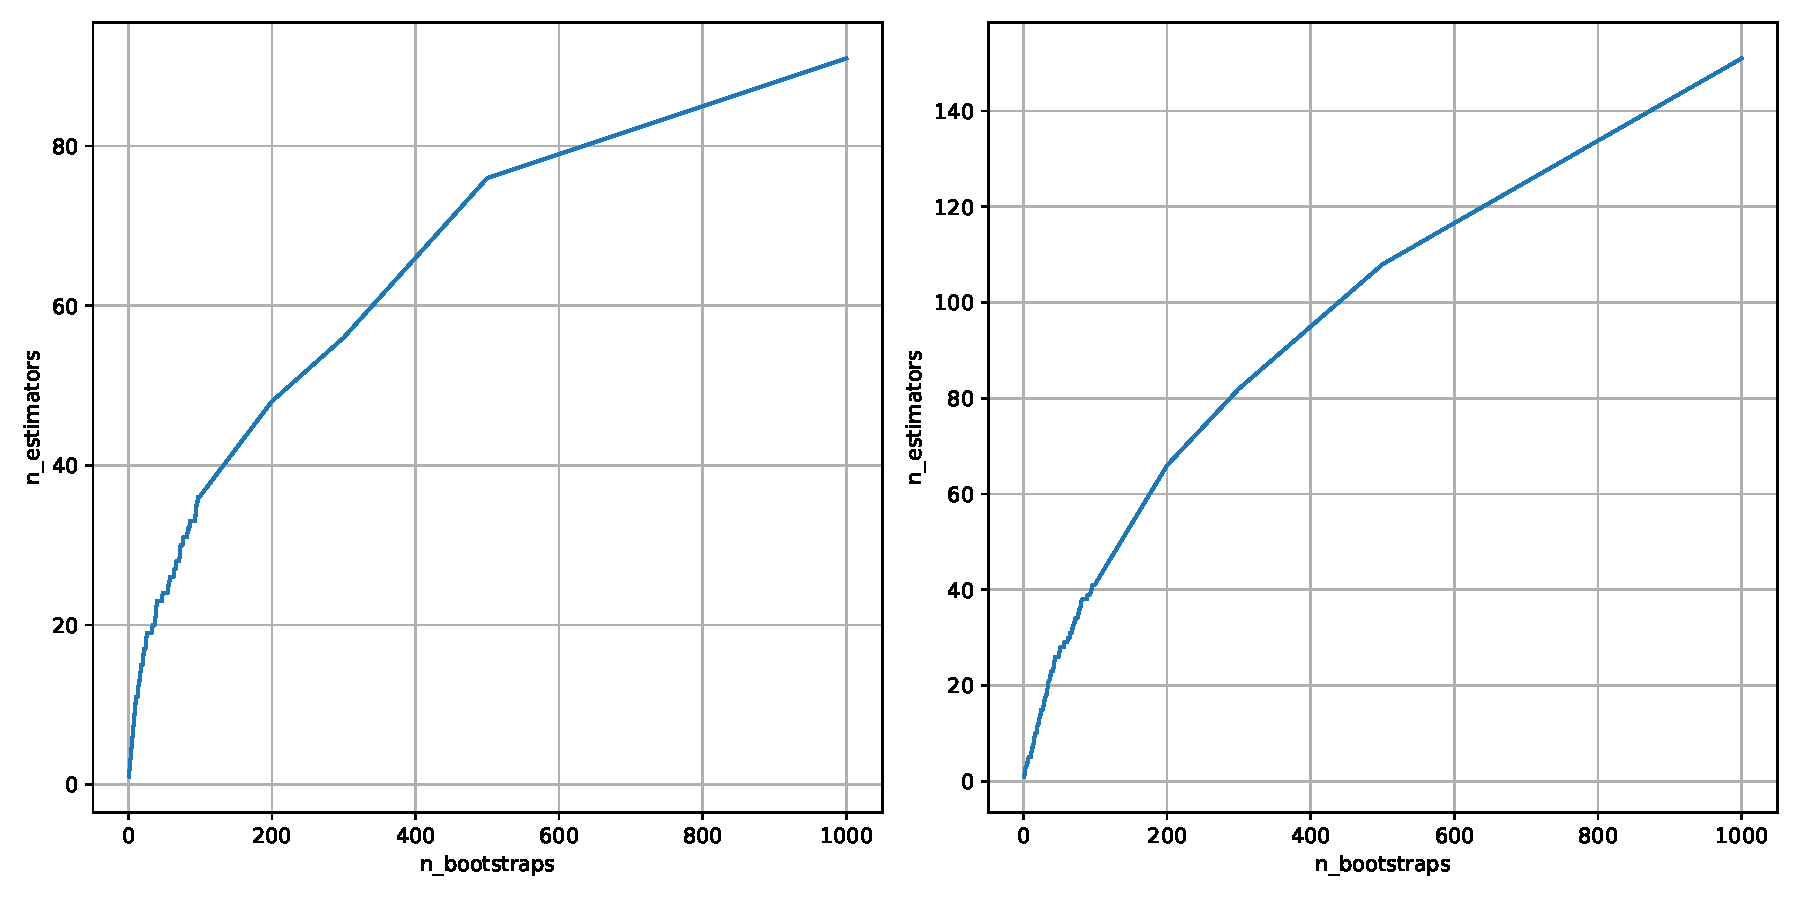
\includegraphics[width=0.8\linewidth]{pictures/n_estimators.pdf}
    \caption{Число уникальных предикторов}
    \label{Pic 3}
\end{figure}\\
По графику [\ref{Pic 3}] можно видеть, что при $1000$ бутстрапирований уникальных предикторов остается порядка $10\%$, следовательно, вариативность ансамбля при дальнейшем наращивании числа бутстрэпов будет изменяться незначительно. 
\newpage
Также построим распределение коэффициента корреляции уникальных предикторов при числе бустрапирований в $1000$.
\begin{figure}[!htb]
    \centering
    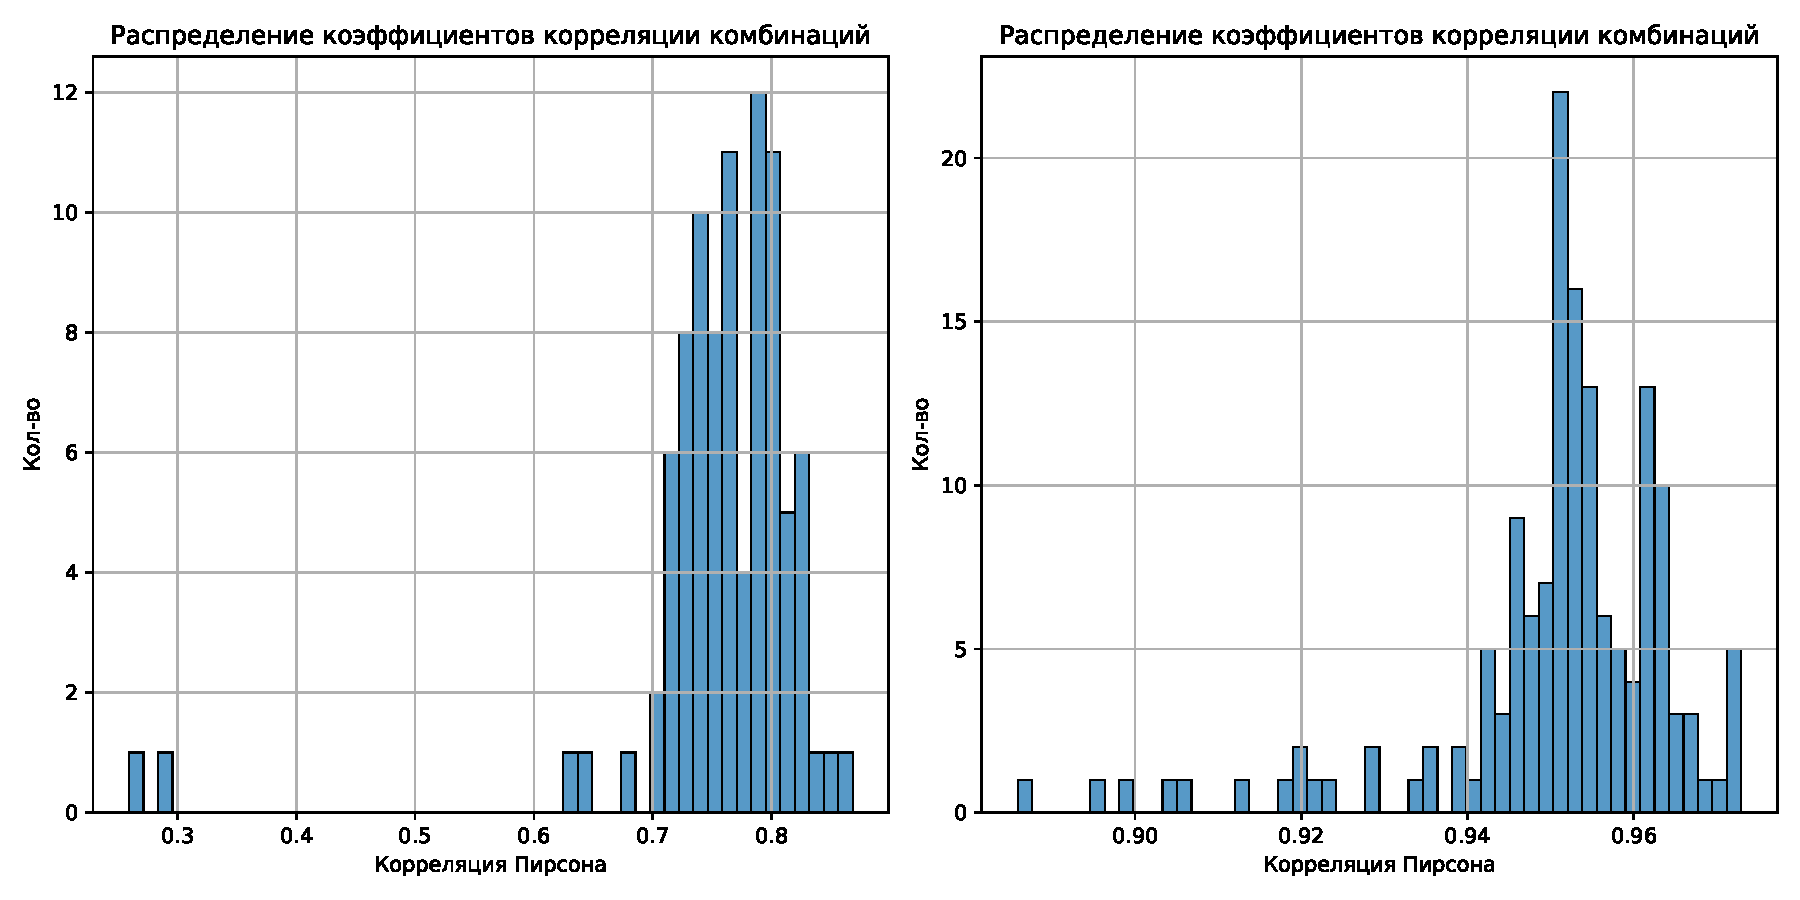
\includegraphics[width=1\linewidth]{pictures/corr_coefs_bootstrap.pdf}
    \caption{Оценка коээфициентов корреляции}
\end{figure}\\
В сравнении с классическим методом среднее значение корреляции смещается в сторону $1$, что обосновывается жадным отбором лучшей комбинации на каждом шаге, но из-за добавления метода случайных подпространств корреляции некоторых комбинаций могут существенно уменьшаться из-за  <<плохих>> признаков в подпространстве. 
\section{Итоги}
В результате работы были приведены необходимые теоретические обоснования для построения модели, основанной на ансамблировании линейных моделей с помощью выпуклых комбинаций с целью максимизации корреляции с целевой переменной. Сам алгоритм был запрограммирован и проверен на реальных данных. Модель показала результаты лучше некоторых уже существующих решений, вошедших в широкое использование. Были проведены исследования полученной модели и более эффективных методов агрегации итогового ансамбля. Помимо классического алгоритма был рассмотрен метод, существенно уменьшающий вычислительные сложности перебора $d!$ комбинаций, основанный на методе случайных подпространств и жадного отбора. В дальнейшем алгоритм можно развить с помощью идеи дивергентного леса, представленной в статье [13].  
\newpage 
\newpage 
\section{Список литературы}
1. Ridge Regression in Practice//Donald W. Marquardt and Ronald D. Snee The American Statistician Vol. 29, No. 1 (Feb., 1975), pp. 3-20.
2. Tibshirani R. Regression shrinkage and selection via the lasso//J.Roy.Stat.Soc.1996.V.58.P.267–288. \\ \\
3. ZouH., HastieT., EfronB., HastieT. Regularization and variable selection via the elastic net//J.Roy.Stat.Soc. 2005. V. 67. No 2. P. 301–320. \\ \\
4. Least Angle Regression//Bradley Efron, Trevor Hastie, Iain Johnstone, Robert Tibshirani The Annals of Statistics 2004, Vol. 32, No. 2, 407–451 \\ \\
5. Relaxed Lasso//Nicolai Meinshausen Computational Statistics & Data Analysis
Volume 52, Issue 1, Pages 374-393 \\ \\
6. A Sparse-group Lasso //Noah Simon, Jerome Ffiedman, Trevor Hhastie, Rob Tibshirani. \\ \\
7. Robust and sparse estimators for Linear Regressions Models//Ezequiel Smucler, V´ıctor J. Yohai arXiv:1508.01967v4 \\ \\
8. Stacked regressions//Breiman L. (1996) \\ \\
9. Random forests – random features//Breiman L. (1996) \\ \\
10. Ensembles of Regularized Linear Models//Anthony Christidis, Laks V.S. Lakshmanan, Ezequiel Smucler, Ruben Zamar (2001)\\ \\
11. А. А. Докукин, О. В. Сенько, “Регрессионная модель, основанная на выпуклых комбинациях, максимально коррелирующих с откликом”, Ж. вычисл. матем. и матем. физ., 55:3 (2015), 530–544; Comput. Math. Math. Phys., 55:3 (2015), 526–539 \\ \\
12. Senko O., Dokukin A. Optimal forecasting based on convex correcting procedures // New Trends in Classifica* tion and Data Mining. ITHEA, Sofia, 2010. P. 62–72. \\ \\
13. Diversified Random Forests Using Random Subspaces//Khaled Fawagreh, Mohamed Medhat Gaber, Eyad Elyan. \\ \\
14. Bayesian non-linear modeling for the prediction competition//David J.C. MacKay, Cavendish Laboratory. \\ \\
15. Sparse Bayesian Learning and the Relevance Vector Machine//David J. C. MacKay, Michael E. Tipping. \\ \\
16. Random generalized linear model: a highly accurate and interpretable ensemble predictor.//Song, L., Langfelder, P., and Horvath, S. (2013).  BMC bioinformatics, 14(1):5. \\ \\
17. The cluster elastic net for high-dimensional regression with unknown variable grouping.//Witten D., Shojaie A., Zhang F. (2014). Technometrics, 56(1):112–122. \\ \\
18. Asymptotic properties of subspace estimators. // D. Bauer. Automatica, 41:359–376, 2005. \\ \\
19. The Dantzig selector: statistical estimation when p is much larger than n.// Candes and T. Tao. Annals of Statistics, 35:2313–2351, 2007. \\ \\
20. Aggregating regression procedures to improve performance.//Yang, Y. (2004). Bernoulli, 10(1):25–47.
\end{document}
